

%\documentclass[a4paper]{article}
\documentclass[reprint,amsmath,amssymb,aps,prl,superscriptaddress]{revtex4-1}
%% Language and font encodings
\usepackage[english]{babel}
%\usepackage[utf8x]{inputenc}
%\usepackage[T1]{fontenc}

%% Sets page size and margins
%\usepackage[a4paper,top=3cm,bottom=2cm,left=3cm,right=3cm,marginparwidth=1.75cm]{geometry}

%% Useful packages
\usepackage{amsmath}
\usepackage{graphicx}
\usepackage[colorinlistoftodos]{todonotes}
\usepackage[colorlinks=true, allcolors=blue]{hyperref}
\usepackage{lineno}
\linenumbers
\usepackage{multirow}
\usepackage{enumitem}

\begin{document}

\title{Pixel Readout Technology for Liquid Argon Time Projection Chambers}

\author{Author A}

\begin{abstract}
Abstract
\end{abstract}

\maketitle

%%%%%%%%%%%%%%%%%%%%%%%%%%%%%%%%%%%%%%%%%%%%%%%%%
\section{Introduction}\label{sec:intro}
%%%%%%%%%%%%%%%%%%%%%%%%%%%%%%%%%%%%%%%%%%%%%%%%%
Large scale noble element time projection chambers (TPC's) play a central role in many aspects of high energy physics experiments. As charged particles traverse the bulk material they produce ionization electrons and scintillation photons. An external electric field allows the ionization electrons to drift towards the anode of the detector and be collected on charge sensitive readout. The combined measurement of the scintillation light, providing the $t_0$, and the arrival time of the ionization charge allows for the 3D reconstruction of the original charged particle topology within TPC. Thus the TPC provides a fully active tracking detector with calormetric reconstruction capabilities without instrumenting the bulk volume of the detector.

More recently, the advances in large scale liquid noble TPC's to drift electrons over many meters has lead to a rise in their use as neutrino detectors to study of neutrino oscillations over relatively short baselines ($<1$~km) and long baselines ($>1000$~km). Specifically, Liquid Argon Time Projection Chambers (LArTPCs) \cite{TPC1, TPC2, TPC3} offer fine-grain tracking as well as powerful calorimetry and particle identification capabilities making them ideal detectors for studying neutrino-nuclei interactions. 

The standard method for reading out the ionization charge in a LArTPC relies on the use of consecutive planes of sensing wires to measure two of the three space coordinates. This method was used for ICARUS \cite{ICARUS} and MicroBooNE \cite{uBooNE}, and was also adopted as a baseline configuration for the Deep Underground Neutrino Experiment (DUNE) \cite{DUNE} far detector. Although the concept is proven and gained considerable interest in the community, it has an intrinsic limitation in resolving ambiguities, which result in making the event reconstruction difficult in some cases. In addition, the construction and mounting of massive anode plane assemblies to host the wire planes poses difficult engineering challenges and is considerably expensive. For these reasons, a non-projective readout would have many advantages. 

Such a readout scheme has been utilized in many gas based TPC but was not considered viable LArTPC's because of the number of readout channels and power consumption requirements on existing LArTPC readout technologies. The number of pixels for equal spatial resolution will be two or three orders of magnitude higher than the number of corresponding sense wires, with an analogous increase of the number of signal channels, data rates and power dissipation. This would make such a solution untenable except for very small detectors. A truly transformative step forward for future LArTPCs is the ability to build a fully pixelated low power charge readout.

The endeavour to build a low power pixel based charge readout for use in LArTPC's has independently inspired two research groups to pursue complimentary approaches to solving this problem. The LArPix \cite{} and Q-Pix \cite{} consortium's have undertaken the challenge of the research and development necessary to realize a pixel based readout. This document is meant to provide an overview of both the LArPix and Q-Pix approaches and outline design philosophies, complementarity and synergies to their approaches. The paper is laid out to first provide the motivation in the current experimental landscape as well as give reference to previous work which has been pursued. Next, an overview of the LArPix and Q-Pix designs is given with a dedicated section to their complimentarity. We conclude with an outline of ongoing R\&D being pursued by both groups.    

%%%%%%%%%%%%%%%%%%%%%%%%%%%%%%%%%%%%%%%%%%%%%%%%%
\subsection{Motivation}\label{sec:motive}
%%%%%%%%%%%%%%%%%%%%%%%%%%%%%%%%%%%%%%%%%%%%%%%%%
The next generation long-baseline neutrino experiments aim to answer the questions of the exact ordering of the neutrino mass states, known as the mass hierarchy, as well as the size of the CP-violating phase $\delta$. These, as yet unknown quantities, remain one of the last major pieces of the Standard Model of particle physics and offer the opportunity to answer such fundamental questions as ``what is the origin of the matter/antimatter asymmetry in the universe?'' and ``do we understand the fundamental symmetries of the universe?''. By measuring the asymmetry between appearance of electron neutrinos from a beam of muon neutrinos ($P(\nu_{\mu} \rightarrow \nu_{e}$)) compared to the appearance of electron antineutrinos from a beam of muon antineutrinos and $P(\bar{\nu}_{\mu} \rightarrow \bar{\nu}_{e}$)) as well as the precise measurement of the $\nu_{e}$ energy spectrum measured at the far detector, both the CP violating phase ($\delta_{CP}$) and the mass hierarchy can be measured in the same experiment .

The Deep Underground Neutrino Experiment (DUNE) aims to accomplish these measurments and will be the US flagship high energy physics experiment for the next 15-20 years. DUNE will require three essential components: \textbf{1) A high power neutrino beam} designed to provide sufficient intensity and appropriate energy range to enhance the sensitivity to the first and second oscillation maximum. The beam is to be sign-selected to provide separate neutrino and antineutrino beams with high purity to enable measurement of CP violation, the neutrino mass hierarchy, and precision oscillation measurements. \textbf{2) A precision near detector} measuring the un-oscillated neutrino spectrum for the CP-phase and mass hierarchy measurement, and \textbf{3) Large mass underground detectors} consisting of four 10 kT liquid argon time projection chambers deployed 4850 feet underground in order to reduce the number of cosmic rays in time with the neutrino beam. 

The physics requirement on the near detector and far detector necessitate a difference in the approach to each. The primary role of the DUNE near detector (DUNE-ND) system is to characterize the energy spectrum and the composition of the neutrino beam at the source, in terms of both  ${\nu}_{\mu} / \bar{\nu}_{\mu}$ and ${\nu}_{e} / \bar{\nu}_{e}$, and to provide measurements of neutrino interaction cross sections. Systematics associated with the near/far extrapolation can be minimized by having a highly capable near detector that can independently constrain the neutrino cross-section models, neutrino flux, and energy resolution. DUNE-ND is thus envisioned to be formed from various components which serve individual and overlapping functions. At the core of the DUNE-ND complex will be a new LArTPC in order to provide the same target nucleus and similar functionality with the far detector. The DUNE far detectors will have to be capable of high efficiency precision ${\nu}_{\mu} / \bar{\nu}_{\mu}$ and ${\nu}_{e} / \bar{\nu}_{e}$ identification and energy measurements to provide a definitive measurement of the CP-phase and mass hierarchy as well as being capable of detecting low-energy neutrinos originating from supernovae bursts and have the ability to detect the signature of baryon number violation (via proton decay or neutron/anti-neutron oscillations) \cite{Abi:2018dnh}.

The operating conditions of the LArTPC in the DUNE near detector are much different then that of the far detector.  The high intensity neutrino beam seen by the near detector means there will be multiple overlapping neutrino interactions within the liquid argon volume, as shown in Figure \ref{fig:ND-FDEvents}. Thus a smaller, segmented, and modular TPC design with optically isolated modules and pixel based readout is envisioned. This is in stark contrast to the operating conditions of the LArTPC far detector which expect to see $\sim 4$ beam-events / day / 10-kTon module. This suggests a design of large uninterrupted modules with long drifts and maximal coverage for the pixel design. 



\begin{figure}[htb]
  \begin{center}
    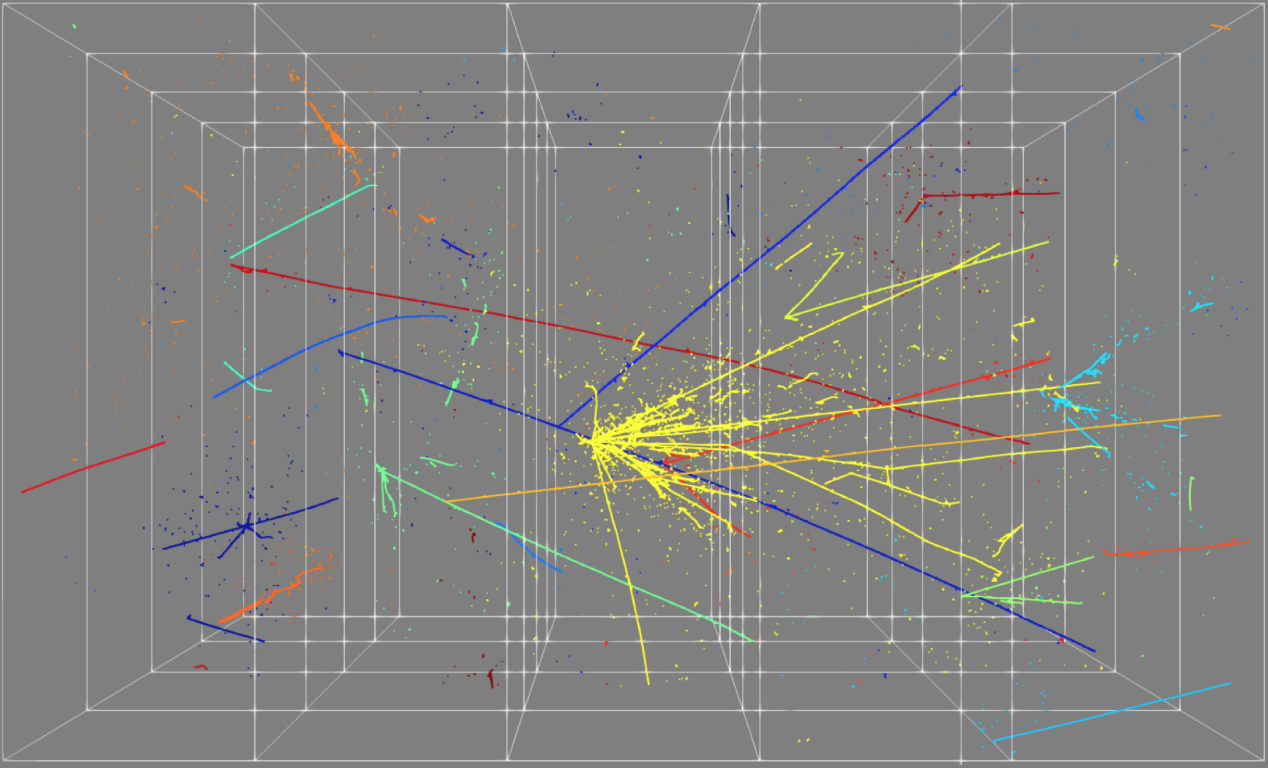
\includegraphics[width=0.35\textwidth]{ND.png}
    \caption{(Top) An event display showing a typical multiple neutrino interaction event as well as rock muons expected in the liquid argon DUNE near detector. The various interactions are grouped by color. (Bottom) An event display  of a 10 kTon DUNE far detector module showing a typical neutrino interaction. The level of different activity seen by the two LArTPC's can clearly be seen.\label{fig:ND-FDEvents}}
  \end{center}
\end{figure}

Desired physics signature is much different with ND having GeV scale physics of the interactions being the target for the near detector measurements while the FD has to be ready for discovery and with lower thresholds may open up the opportunity for atmospheric neutrinos as well!

%%%%%%%%%%%%%%%%%%%%%%%%%%%%%%%%%%%%%%%%%%%%%%%%%
\subsection{Previous Work}\label{sec:background}
%%%%%%%%%%%%%%%%%%%%%%%%%%%%%%%%%%%%%%%%%%%%%%%%%

Information about Bern's previous efforts (analog multiplexed signals) and PixLAr run done in 2017 

%%%%%%%%%%%%%%%%%%%%%%%%%%%%%%%%%%%%%%%%%%%%%%%%%
\section{Current Efforts}\label{sec:CurrentEfforts}
%%%%%%%%%%%%%%%%%%%%%%%%%%%%%%%%%%%%%%%%%%%%%%%%%

The need for multiple approaches (Near detector and far detector)

%%%%%%%%%%%%%%%%%%%%%%%%%%%%%%%%%%%%%%%%%%%%%%%%%
\subsection{Overview of LArPix}\label{sec:LArPixOverview}
%%%%%%%%%%%%%%%%%%%%%%%%%%%%%%%%%%%%%%%%%%%%%%%%%

%%%%%%%%%%%%%%%%%%%%%%%%%%%%%%%%%%%%%%%%%%%%%%%%%
\subsection{Overview of Q-Pix}\label{sec:QPixOverview}
%%%%%%%%%%%%%%%%%%%%%%%%%%%%%%%%%%%%%%%%%%%%%%%%%

%%%%%%%%%%%%%%%%%%%%%%%%%%%%%%%%%%%%%%%%%%%%%%%%%
\section{Synergies}\label{sec:CurrentEfforts}
%%%%%%%%%%%%%%%%%%%%%%%%%%%%%%%%%%%%%%%%%%%%%%%%%


%%%%%%%%%%%%%%%%%%%%%%%%%%%%%%%%%%%%%%%%%%%%%%%%%
\section{Ongoing R\&D}\label{sec:CurrentEfforts}
%%%%%%%%%%%%%%%%%%%%%%%%%%%%%%%%%%%%%%%%%%%%%%%%%

\end{document}
